%Vyberte nejvhodnější variantu na trhu dostupného řešení a konfrontujte ji s praxí ve vybrané organizaci. 
\section{Výběr nejvhodnější varianty}

Předchozí analýzy prokázaly, že neexistuje řešení, které by dokázalo zastřešit všechny případy užití vlastních zařízení ve firemním prostředí. Proto tato práce bude dále dělit BYOD podle typu zařízení a to na mobilní zařízení jako jsou mobilní telefony či tablety a notebooky.

\section{Výběr řešení pro mobilní telefony a tablety}

\todo{Proc je potreba EMM? Viz specifikace projektu Good}

Trh nástroji v posledních letech výrazně rostl, zároveň se však konsilidoval. \todo{citace https://theictscoop.com/airwatch-consolidates-emm-leadership-in-latest-idc-report-6622602febde   } V grafech \ref{EMM:podil2015} a \ref{EMM:podil2016} je vidět nárůst trhu s EMM mezi lety 2014 a 2015 z 1,4 miliardy dolarů na 1,8 miliardy dolarů, tedy o 26,9 \%. Zároveň je vidět zvyšování tržního podílu velkých hráču. Výrazný vliv měla také akvice společosti Good Technology společností BlackBerry.

 
  \begin{figure}[h]
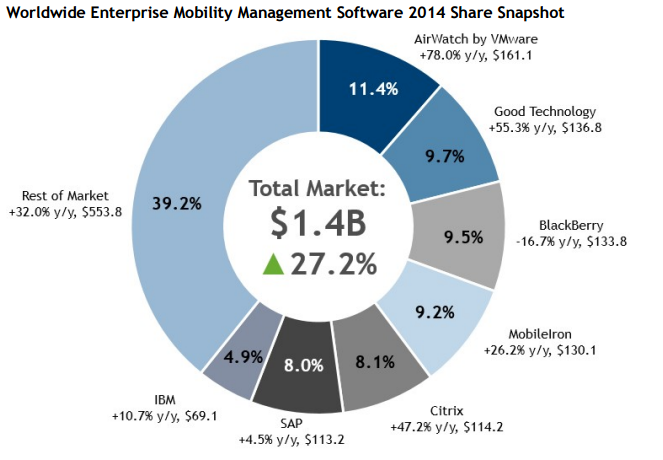
\includegraphics[width=13cm]{img/IDC_EMM}
\caption{Podíl na trhu jednotlivých poskytovatelů EMM v roce 2014 podle IDC Převzato z \cite{}} 
\label{EMM:podil2015}
\centering
\end{figure}\todo{citace http://www.idc.com/getdoc.jsp?containerId=US40430516  }

  \begin{figure}[h]
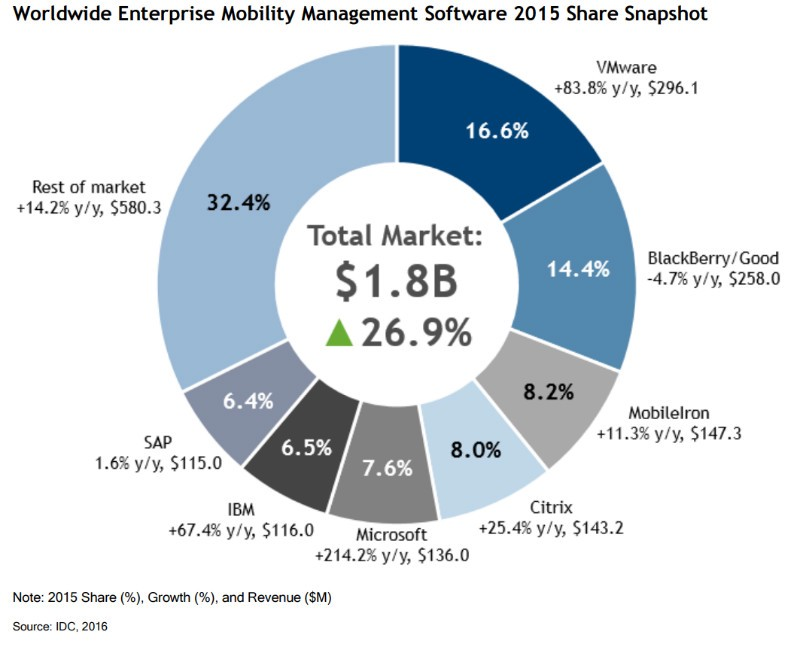
\includegraphics[width=13cm]{img/IDC_EMM_2016}
\caption{Podíl na trhu jednotlivých poskytovatelů EMM v roce 2015 podle IDC Převzato z \cite{}} 
\label{EMM:podil2016}
\centering
\end{figure}\todo{citace https://theictscoop.com/airwatch-consolidates-emm-leadership-in-latest-idc-report-6622602febde   }

Modle magazínu CIOReview bylo v roce 2016 pro BYOD nejslibnějších následujících dvacet poskytovatelů software: Accelion, API Systems, Cyber adAPT, Ericom Software, Excelerate Systems, GSG Telco, High Point Solutions, LANDESK Software,  Mathe, MobileIron, MobilityLab, Movius, RES Software, Sirama Consulting, Skycure, Storgrid, Tangoe, Tyfone, VmWare AirWatch, Zix Corporation.

Některé z nich jsou však příliš úzce zaměřené, či jsou pouze minoritními hráči na trhu. Analýza společnosti Gartner \cite{Gartner_EMM_2016} z roku 2016 pro EMM rozděluje jednotlivé poskytovatele dle jejich postavení na trhu a zároveň zohledňuje jejich schopnost zohlednit v produktu aktuální požadavky trhu a nasměrování produktu k budoucím potřebám zákazníků. Tyto kritéria shrnuje společnost Gartner jako osy "schopnost vykonat" a "úplnost vize" ve svém grafu nazývaném magic quadrant. \ref{EMM:quadrant}

 \begin{figure}[h]
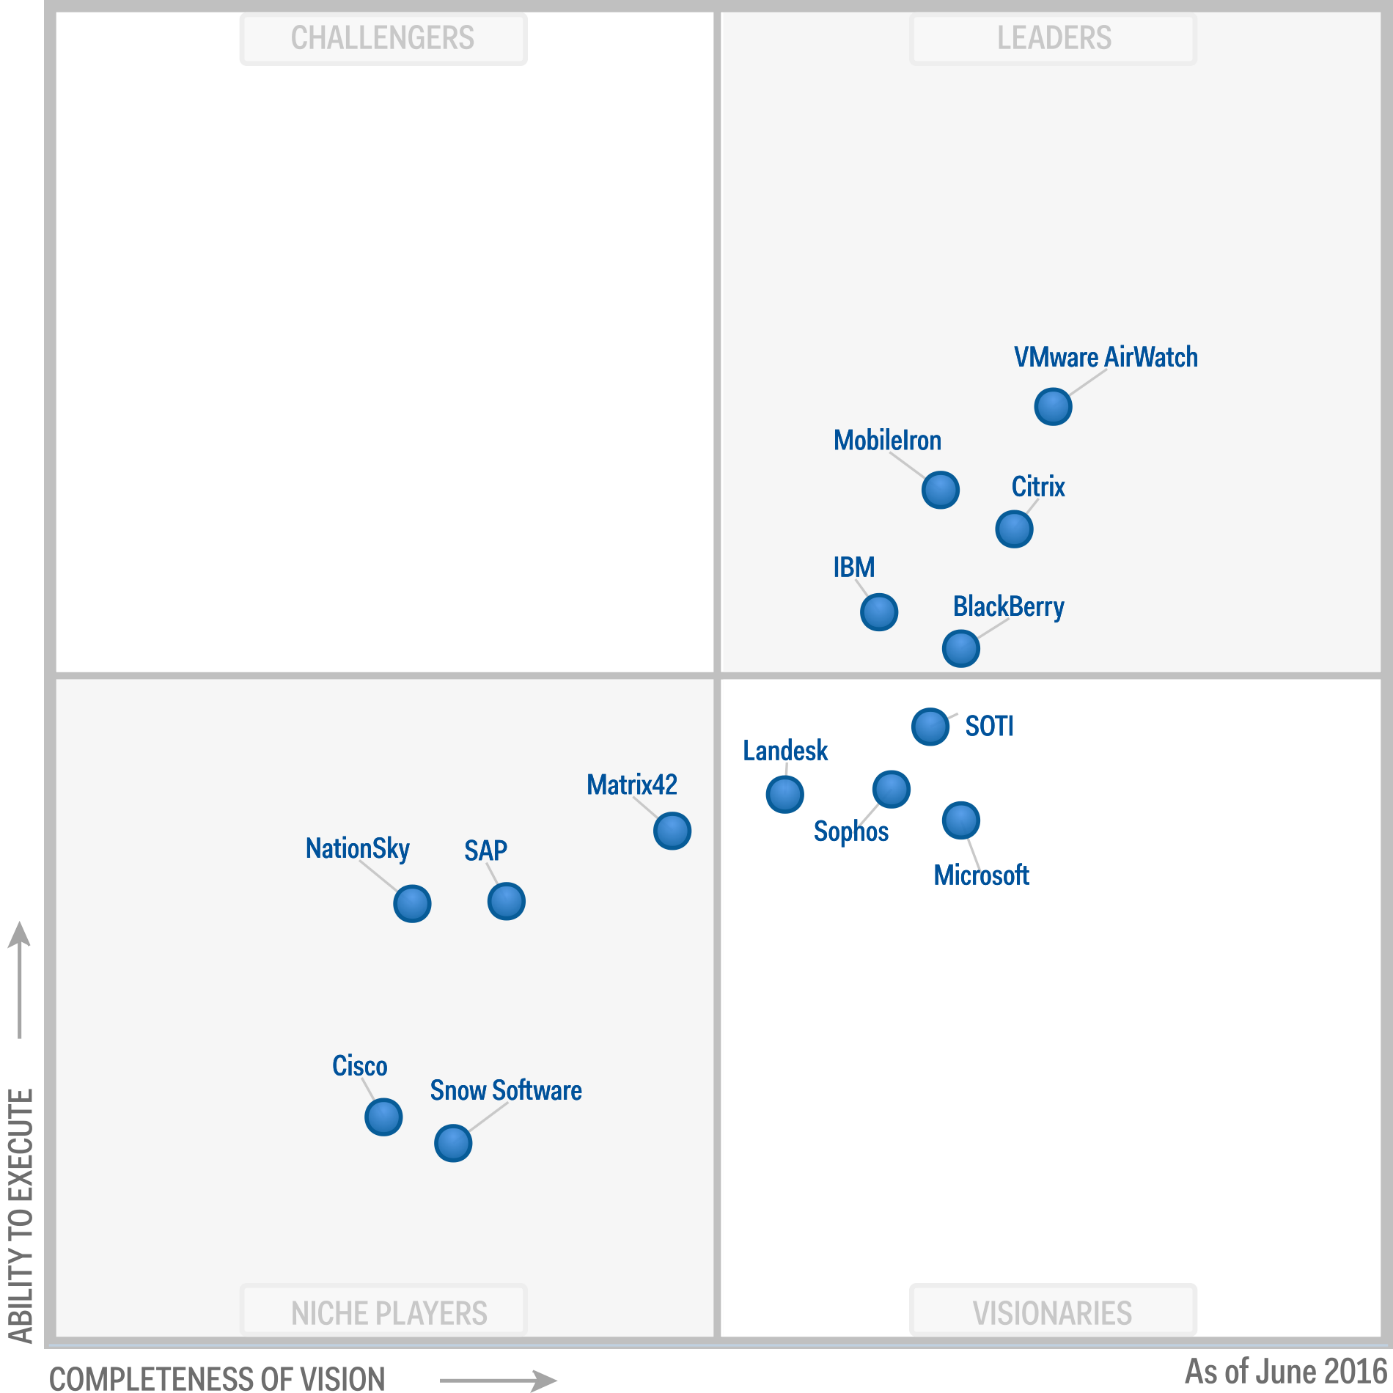
\includegraphics[width=13cm]{img/Gartner_EMM}
\caption{Gartner Magic quadrant. Převzato z \cite{Gartner_EMM_2016}} 
\label{EMM:quadrant}
\centering
\end{figure}\todo{citace}
 %\missingfigure{magic quarter}
 
Následující společnosti se nacházejí v kvadrantu lídrů:

\subsubsection{VMWare Airwatch}
\subsubsection{MobileIron}
\subsubsection{Citrix}
\subsubsection{IBM}
\subsubsection{BlackBerry}
BlackBerry nyní prodává svůj nástroj jako Good Secure EMM Suite. Skládá se z BES12, Good collaboration apps, Good dynamics a WatchDox Enterprise. Produkty pod značkou Good a WatchDox získala Blacberry akvizicemi které byly dokončeny v roce 2015. \todo{citace http://global.blackberry.com/en/company/newsroom/press?id=1998017} \todo{http://global.blackberry.com/en/company/newsroom/press?id=1946553}



\section{Výběr řešení pro notebooky}


%Konzultujte navrhované řešení se zástupci vybrané organizace a stanovte doporučení pro nasazení. 
\section{Hodnocení navrhované varianty zástupci KB}

%Navrhněte nasazení řešení BYOD. 
\section{Návrh řešení}


%Zhodnoťte uskutečnitelnost řešení a analyzujte benefity a rizika spojená se zavedením navrženého konceptu.
\section{Analýza navrženého řešení}